
\section{Headtracking}

Ziel des Headtrackings ist es, die Kopforientierung des Fahrers --auch bei bewegtem \todo{``fahrendem'' statt ``bewegendem''?} Fahrzeug-- sowohl relativ zum Fahrzeug als auch in Weltkoordinaten anzugeben. Unter Orientierung wird hier die Drehung entlang der X (\emph{Roll}), Y (\emph{Pitch}) und Z-Achse (\emph{Yaw}) verstanden.

Dazu wird die Inertialsensorik der \ac{AR}-Brille, bestehend aus zwei Gyroskopen, Beschleunigungssensor und Magnetometer, ausgewertet (Abs. \ref{headtracking_imu_subsec}).
Diese Daten werden mit einem geeigneten Filter-Algorithmus fusioniert (Abs. \ref{headtracking_fusion_subsec}).
Die Kompensation der Eigenbewegung des Fahrzeugs wird in Abs. \ref{headtracking_marker_subsec} behandelt.


\subsection{Inertialsensoren}
\label{headtracking_imu_subsec}


\subsubsection{Gyroskop}

Das in der Brille enthaltene Gyroskop misst Winkelgeschwindigkeiten in
$\omega = [{Grad \over Sekunde}]$ bei Drehungen um die X, Y und Z-Achse. Durch
die Integration der Winkelgeschwindigkeiten über die Zeit kann die
Orientierung der Brille bestimmt werden.  

Die IMU der Brille enthält zwei
Gyroskope, ein \emph{High Bandwidth} Gyrosokp (HBW) sowie ein
\emph{Low Bandwidth} Gyroskop (LBW). Die Gyroskope unterscheiden sich
hinsichtlich der Genauigkeit und des Wertebereiches. Das HBW-Gyroskop
hat hierbei einen größeren Wertebereich, jedoch die geringere
Genauigkeit.

Die Rohdaten des Sensors enthalten einen konstanten Versatz, so dass bei
stationärer Brille eine Geschwindigkeit $\omega \neq 0$ gemessen wird. Dieser
Versatz wird \emph{Bias} genannt, und muss in einem stationären
Kalibriervorgang ermittelt werden. Während des Kalibriervorganges wird
der Bias gemittelt, dieser wird nach Beendigung des Kalibriervorganges von den
Rohdaten abgezogen. Abb. \ref{fig-bias-correction} zeigt die Daten vor und nach der
Bias-Korrektur.

\todo{Abbildung Bias-Korrektur}

Desweiteren unterliegen die Sensordaten einem Rauschen. Daher wird als
nächster Schritt ein Tiefpassfilter verwendet, um dieses Rauschen zu
reduzieren. In unserem Fall hat sich ein Mittelwertfilter mit einer 
Fenstergröße von 5 als praktikabel erwiesen. Je höher die Fenstergröße gewählt wird,
desto stärker werden die Rohdaten geglättet, damit steigt jedoch auch
die Verzögerung der Daten.  Siehe hierzu Abb. \ref{fig-lowpass-delay}.

\todo{Abbildung Lowpass}

Zur Fusionierung des HBW- und LBW-Gyroskops kommt ein einfaches
Schwellwertverfahren zum Einsatz. Die Wertebereiche der Gyroskope sind
in Tabelle \ref{tab:ranges-gyros} aufgeführt. Beide Gyroskope liefern
einen 12-Bit-Datenwert. Somit stellt ein Zählwert des LBW-Gyroskops eine
kleinere Veränderung dar als beim HBW-Gyroskop, was gleichbedeutend mit
einer höheren Genauigkeit ist.

\begin{table}[position specifier]
  \centering
  \begin{tabular}{ | c | c | c | }
    \hline
    & Min. & Max. \\ \hline
    LBW & -420   & 420   \\ \hline
    HBW & -1680   & 1680   \\
    \hline
  \end{tabular}
  \caption{Wertebereiche der Gyroskop-Sensoren in $[{\degree \over s}]$.}
  \label{tab:ranges-gyros}
\end{table}

%\begin{center}
%  \begin{tabular}{ | c | c | c | }
%    \hline
%    & Min.  $[{\degree \over s}]$& Max. $[{\degree \over s}]$\\ \hline
%    LBW & -420   & 420   \\ \hline
%    HBW & -1680   & 1680   \\
%    \hline
%  \end{tabular}
%\end{center}

Im Wertebereich, welcher von beiden Gyroskopen abgedeckt wird, werden
die Sensordaten gemittelt. Wird der Wertebereich des LBW-Gyroskops
überschritten, wird lediglich der Wert des HBW-Gyroskops
zurückgeliefert. 

%\begin{equation}
%    \omega_{fusioniert} = 
%    \begin{cases}
%        {\omega_{HBW} + \omega_{LBW}} \over 2 & \text{für} |\omega_{HBW}| < 420 \\
%        \omega_{HBW} & \text{sonst}
%%     2x^{2} & \text{f"ur } x \textless 4 \\
%%     2x^{3} + 4^{2} & \text{fur} 4 \ge x \textless 27 \\
%%     3x^{2} \cdot sin(x) & \text{far } x \ge 27 
%   \end{cases}
%\end{equation}

Aus den gefilterten Sensordaten wird daraufhin durch Integration über
die Zeit die Orientierung berechnet. Hierzu wird die Orientierung in einem Quaternion gespeichert, welches nach jeder Sensor-Abtastung aktualisiert wird. Hierbei ist $dt$ die Abtastrate der Gyroskop-Sensoren.

\begin{equation}
    \Delta q = quaternion({\omega_x \over dt}, {\omega_y \over dt}, {\omega_z \over dt}) \\
\end{equation}

\begin{equation}
    q = q * \Delta q
\end{equation}

Die durch das Gyroskop berechnete Orientierung reagiert schnell auf
Änderungen, durch die Integration entseht in jedem Integrationsschritt jedoch ein Fehler, welcher sich summiert. Dieser Fehler wird als \emph{Drift} bezeichnet. In den folgenden Abschnitten wird beschrieben, wie Beschleunigungssensor und Magnetometer verwendet werden können, um diesen Fehler zu kompensieren.


\subsubsection{Beschleunigungssensor}

Der Beschleunigungssensor misst die Gravitation entlang der X, Y und Z-Achse, im Folgenden als $acc_x$, $acc_y$ und $acc_z$ bezeichnet. Anhand dieses Gravitationsvektors kann die Orientierung der Brille bezüglich der horizontalen Ebene bestimmt werden.

Zur Verwendung des Beschleunigungssensors wird zunächst wie auch beim
Gyroskop ein Tiefpassfilter angewendet, um das Rauschen der Rohdaten zu
reduzieren. Dabei wird die gleiche Fenstergröße wie beim Gyroskop
verwendet, da ein ungleicher Wert zu Fehlern bei der späteren Fusion
führen würde. 

% XXX: die umrechung auf m/s2 hab ich mal rausgelassen, die ist ja glaub ich auch garnicht so wichtig und verwirrt den leser nur

Die Orientierung in Roll und Pitch kann direkt aus den Winkeln des Gravitationsvektors berechnet werden.

\begin{equation}
    roll = atan2(acc_y, acc_z)
\end{equation}

\begin{equation}
    pitch = -atan2(acc_x, \sqrt{ {acc_y}^2 + {acc_z}^2 })
\end{equation}

Die so bestimmten Roll und Pitch Werte sind frei von Drift, und können als Stützwerte für die aus den Gyroskopdaten berechneten Orientierungswerte verwendet werden. Jedoch ist zu beachten, dass der Beschleunigungssensor nicht zuverlässig zur Berechnung des Yaw-Winkels verwendet werden kann. Dies liegt darin begründet, dass sich die Sensordaten des Beschleunigungssensors nicht ändern, wenn sich der Sensor parallel zur Erdoberfläche befindet um den Yaw-Winkel gedreht wird.

%  roll = atan2(acc_data[1], acc_data[2]);
%  pitch = -atan2(acc_data[0], sqrt(acc_data[1]*acc_data[1] + acc_data[2]*acc_data[2]));


\subsubsection{Magnetometer}
\label{headtracking_magnetometer_subsubsec}
\begin{figure}
   \centering
   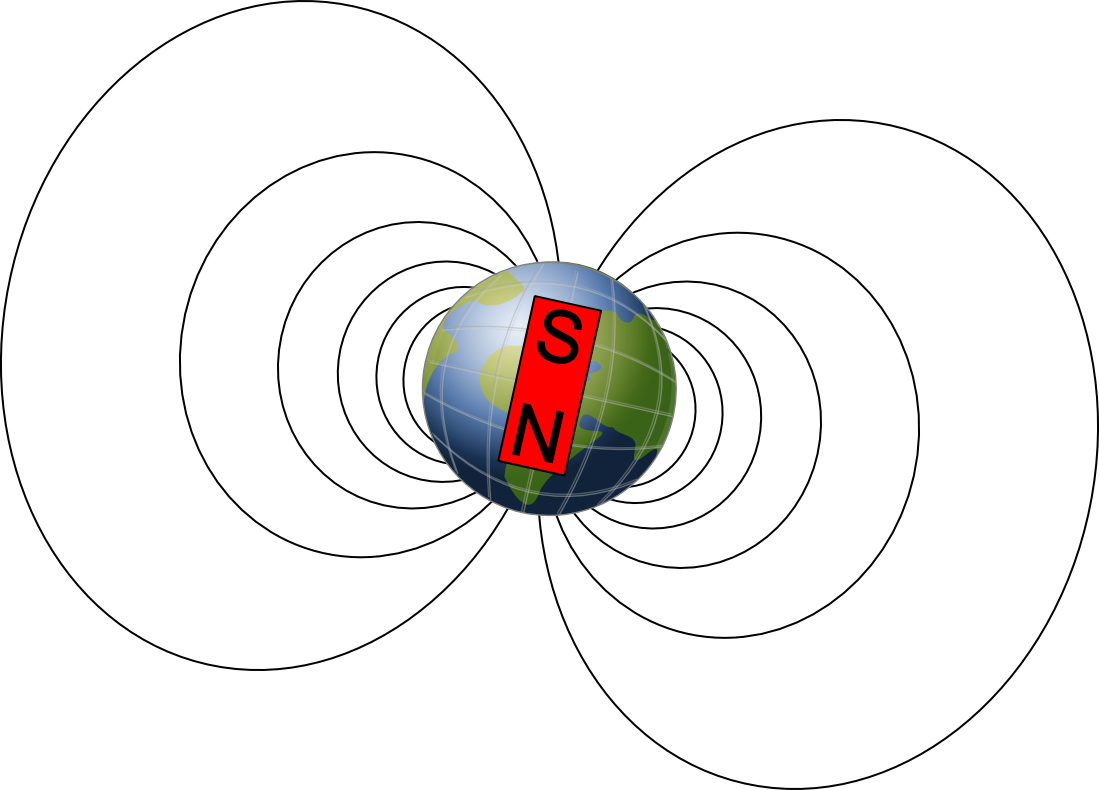
\includegraphics[width=0.3\textwidth]{earth-magnetic-field}
   \caption[mag_world]{Schematische Darstellung des Erdmagnetfelds \cite{mag_world_source}.}
   \label{fig:mag_world}
\end{figure}
\todo{cite Erdmagnetfeld}

\begin{figure}
   \centering
   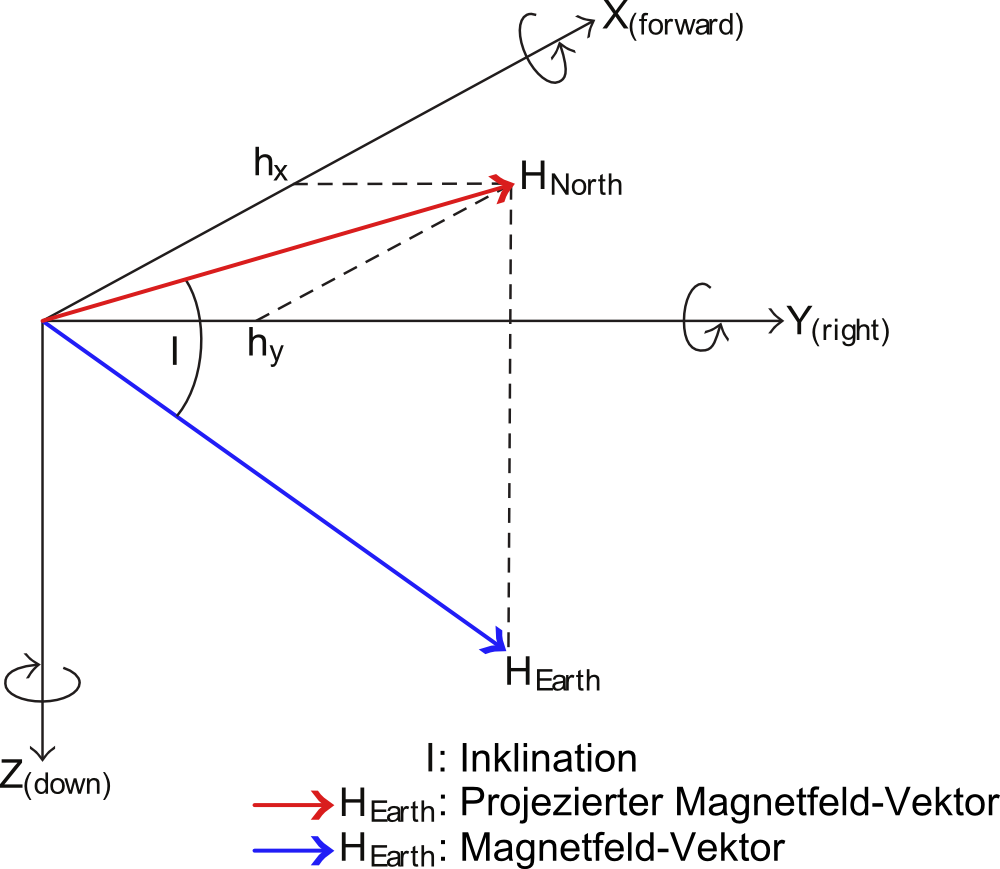
\includegraphics[width=0.3\textwidth]{magnetometer-yaw-calculation}
   \caption[mag_mapping]{Berechungsgrundlage des Magnetfeldvektors}
   \label{fig:mag_mapping}
\end{figure}
Das Magnetometer wird im Rahmen des Praktikums zur Stützung des Yaw-Winkels (Drehung um die Z-Achse des Brillenkoordinatensystem) genutzt.\\
Das verbaute Magnetometer misst in drei Achsen nach dem Funktionsprinzip der Wheatstoneschen Messbrücke \cite{renaudin2010complete} das Erdmagnetfeld.
Dieses Messverfahren führt zum einen zu einer kleinen und kostengünstigen Bauweise.
Zum anderen entstehen aber Messungenauigkeiten, die im Rahmen der Sensorkalibrierung beachtet und ausgeglichen werden müssen.
Gemessen werden die Magnetfeldlinien der Erde, welche in Abbildung \ref{fig:mag_world} dargestellt sind.
Diese sind abhängig von der aktuellen Position auf der Erdoberfläche\footnote{Tatsächlich verändert sich das Erdmagnetfeld auch über die Zeit hinweg.
Diese Änderung kann aber im Rahmen des Praktikums vernachlässigt werden, da es sich um eine sehr kleine Änderung handelt (z. Bsp. für den Praktikumsort Karlsruhe ca. $1^\circ 46$'~$7.8$ arcmin/Jahr im Deklinationswinkel).}.
Sobald das Erdmagnetfeld nicht am Äquator gemessen wird, sondern im Falle unseres Praktikums bei etwa $49^\circ$ geographischer Breite muss der Inklinationswinkel bei der Messung mit beachtet werden, welcher in Abbildung \ref{fig:mag_mapping} mit I beschrieben wird.
Diese Abbildung auf die XY-Ebene wird durch folgende Formel bewerkstelligt:

\begin{equation}
    \varphi = atan2(h_y,h_x)
\end{equation}

Dabei sind $h_x$ und $h_y$ die Anteile des Magnetfeldvektors $H_{Earth}$ in X sowie Y Richtung.

Der gemessene 3D-Magnetfeldvektor ist zunächst unkalibriert und laut der Spezifikation im Datenblatt \todo{cite} einheitenlos.
Daher ist zuerst eine Kalibrierung der gemessenen Werte notwendig um sie weiterverarbeiten zu können. 
Diese Kalibrierung hat zum Ziel einen Kanal-spezifischen Bias auszugleichen. 
Dieser entsteht durch sogenannte \textit{Hard Iron}-Störeffekte, welche durch eigenständige Magnetquellen induziert werden.
Beispiele für diese Störeffekte, sowie die letztlich kalibrierten Daten sind in Abbildung \ref{fig:mag_kugel_plots} als Kugelplots dargestellt.

\begin{figure}[ht]
\centering
\subfigure[Unkalibrierte Magnetometerdaten mit Hard Iron Störeinflüssen]{
    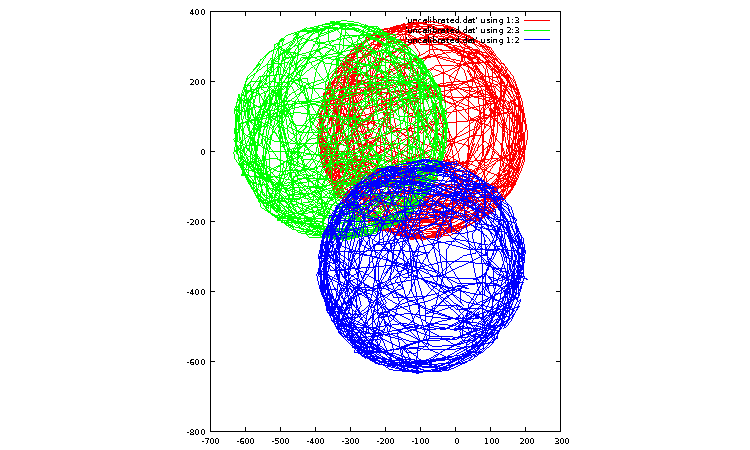
\includegraphics[width=0.3\textwidth]{uncalibrated}
    \label{fig:subfig1}
}
\subfigure[Kalibrierte Magnetometerdaten]{
    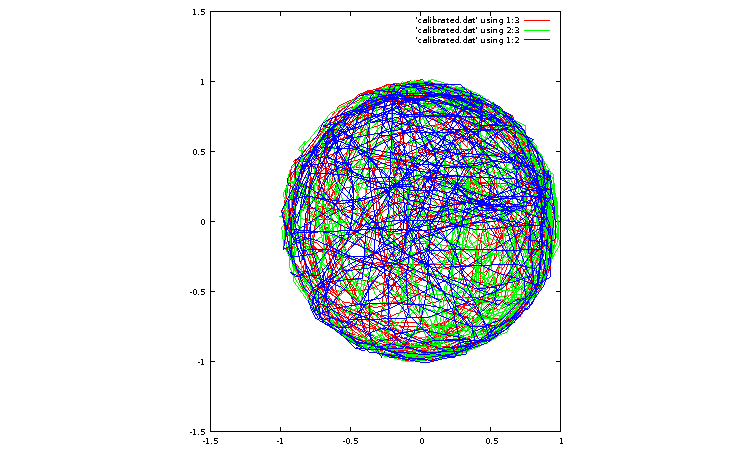
\includegraphics[width=0.3\textwidth]{calibrated}
    \label{fig:subfig2}
}

\caption[]{2D-Sichten auf Kugel aus Magnetometerdaten}
\label{fig:mag_kugel_plots}
\end{figure}


Analog zu den Gyroskopen ist auch beim Magnetometer eine Bias-Korrektur notwendig bevor das \emph{yaw} (aus der Orientierung) gestützt werden kann. Für jede Achse wird unter Berücksichtigung der Min- und Max-Wertes (aus initialer Kalibrierung) der jeweilige Versatz berechnet und verrechnet. In Abbildung \ref{fig:mag_uncalibrated} ist ein Magnetometer im unkalibrierten Zustand zu sehen. Anschließend werden die Werte auf einen Wertebereich von ${[-1, 1]}$ normiert. Eine Abbildung für einen Bias-korrigierten und normierten Daten und somit kalibriertes Magnetometer ist in Abbildung \ref{fig:mag_calibrated} zu entnehmen.       


\begin{figure}[h]
   \centering
   \includegraphics[width=0.65\textwidth]{uncalibrated_circle_with_uncalibrated_lines.pdf}
   \caption[a]{Magnetometer: Unkalibriert}
   \label{fig:mag_uncalibrated}
\end{figure}

\begin{figure}[]
   \centering
   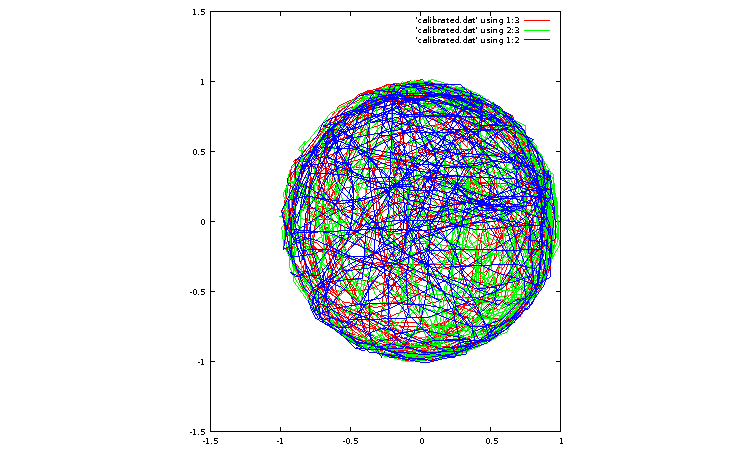
\includegraphics[width=0.6\textwidth]{calibrated.pdf}
   \caption[]{Magnetometer: Kalibriert}
   \label{fig:mag_calibrated}
\end{figure}


%\begin{figure}[h]
%  \centering
%  \subfigure[uncalibrated]{} 
%	\subfigure[calibrated]{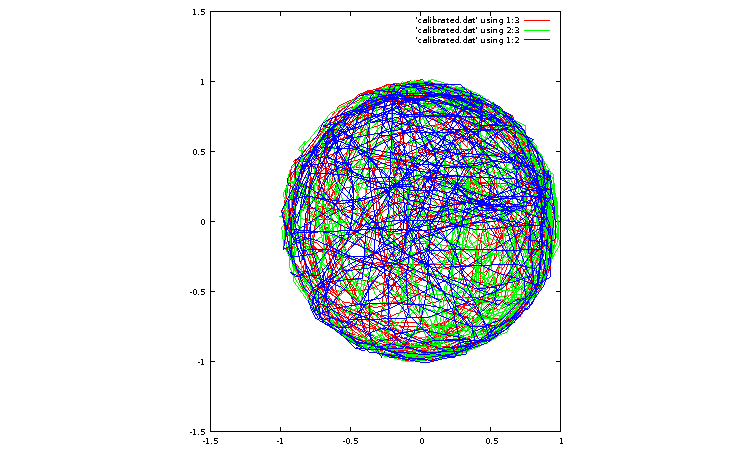
\includegraphics[width=0.4\textwidth]{calibrated.pdf}}
 % \label{fig:mag_uncalibrated}
%	\caption{Magnetometer: Unkalibrierte vs. Kalibrierter}
  %\label{fig:mag_calibrated}
%\end{figure}

Magnetometer-Kreisplots vor/nach Kalibrierung, 
Tiefpassfilter

Magnetometer-Bias-Korrektur (durch Min/Max-Werte), 

Magnetometer-Fehler in Kreisplots
Transformation auf XY Ebene (Algorithmus Ralf)

Im Gegensatz zu den bisher vorgestellten Sensoren wird die Kalibrierung des Magnetometers durch Bewegung durchgeführt.
Ziel ist es, die Wertebereiche in allen drei Achsen zu erfassen.
Dafür wird die Brille in allen Achsen um mindestens $360^\circ$ gedreht, um die minimalen und maximalen Werte zu registrieren. 
Somit kann eine gemäß nachfolgender Formel durchgeführt werden:

\todo{Formel nachschauen}
\begin{equation}
    v_c = ...
\end{equation}

Des weiteren wurden die Daten noch durch einen Tiefpassfilter geglättet sowie auf einen Wertebereich von $[-1,1]$ abgebildet.

Störeinflüsse ansprechen

Stützungsalgorithmus von Ralf